\documentclass[11pt]{article}
\usepackage[utf8]{inputenc}
\usepackage[T1]{fontenc}
\usepackage{calc}
\usepackage{tabu}
\usepackage{tikz}
\usepackage{array}
\usepackage{xcolor}
\usepackage{ifthen}
\usepackage{pgffor}
\usepackage{etoolbox}
\usepackage{fancyhdr}
\usepackage{lastpage}
\usepackage{moresize}
\usepackage{ragged2e}
\usepackage{enumerate}
\usepackage{fontawesome5}
\usepackage{contour,ulem}
\usepackage[scaled]{helvet}
\usepackage{enumitem, pifont}
\usepackage{booktabs, multirow}
\usepackage[hidelinks]{hyperref}
\usepackage{multicol, multicolrule}
\usepackage[absolute,overlay]{textpos}
\usepackage[a4paper, left=2cm, right=2cm, top=1.5cm, bottom=1.5cm]{geometry}



% ---------------------------------------------------------------------------- %
%                                    OPTIONS                                   %
% ---------------------------------------------------------------------------- %
\renewcommand*\familydefault{\sfdefault} % Force the sans-serif version of any font used
\usetikzlibrary{calc,positioning,backgrounds,matrix,shapes,decorations}
\SetMCRule{extend-fill=false}



% ---------------------------------------------------------------------------- %
%                                    LENGTHS                                   %
% ---------------------------------------------------------------------------- %
\newlength\margin\setlength\margin{0.5cm}
\newlength\sidewidth\setlength\sidewidth{0.33333\paperwidth-2\margin}
\newlength\mainwidth\setlength\mainwidth{\paperwidth-4.5\margin-\sidewidth}
\newlength\anglesize\setlength\anglesize{0.7cm}
\newlength\topheight\setlength\topheight{\sidewidth}
\newlength\profilesize\setlength\profilesize{0.7\topheight}

\setlength{\parindent}{0mm} % Suppress paragraph indentation



% ---------------------------------------------------------------------------- %
%                                    COLORS                                    %
% ---------------------------------------------------------------------------- %
\definecolor{Black}{HTML}{353535}
\definecolor{White}{HTML}{FFFFFF}
\definecolor{DarkGreen}{HTML}{252e25}
\definecolor{GreenIT}{RGB}{76, 175, 80}

\newcommand{\DefineColorMacros}[5] {%
    \def\ColorTextSide{#1}
    \def\ColorTextMain{#2}
    \def\ColorHighlight{#3}
    \def\ColorBackground{#4}
    \def\ColorOther{#5}
    \color{\ColorTextMain} % Default
}

\DefineColorMacros{White}{Black}{GreenIT}{Black}{DarkGreen}



% ---------------------------------------------------------------------------- %
%                              FRONT PAGE SECTIONS                             %
% ---------------------------------------------------------------------------- %
\newenvironment{TopBar}[1]
{\begin{textblock*}{\mainwidth} (\sidewidth+3\margin,\margin-0.4cm)\begin{center}\color{#1}}
{\end{center}\end{textblock*}}

\newenvironment{MainPart}
{\begin{textblock*}{\mainwidth} (\sidewidth+3\margin,\topheight+3\margin-0.4cm)\begin{center}}
{\end{center}\end{textblock*}}

\newenvironment{SideBar}[2] {% Background color, Text color
  \begin{tikzpicture}[remember picture,overlay]% put text anywhere    
    \fill[fill=#1, shift={(current page.north west)}] % side and top background
    (0,-\paperheight) -- (0,-\anglesize) --
    (\anglesize,0) -- (\paperwidth,0) --
    (\paperwidth,-\topheight-2\margin) --
    (\sidewidth+2\margin+\anglesize,-\topheight-2\margin) --
    (\sidewidth+2\margin,-\topheight-2\margin-\anglesize) --
    (\sidewidth+2\margin,-\paperheight) --
    cycle;
    \draw [draw=#1, shift={(current page.north west)}, very thick]
    (\paperwidth-0.5\margin,-\topheight-3\margin) --
    (\paperwidth-0.5\margin,-\paperheight+0.5\margin+0.5\anglesize) --
    (\paperwidth-0.5\margin-0.5\anglesize,-\paperheight+0.5\margin) --
    (\sidewidth+3\margin,-\paperheight+0.5\margin);
  \end{tikzpicture}%
  \begin{textblock*}{\sidewidth} (\margin,\topheight+3\margin-0.4cm)
    \begin{center}\color{#2}}{\end{center}
  \end{textblock*}
}



% ---------------------------------------------------------------------------- %
%                                    PICTURE                                   %
% ---------------------------------------------------------------------------- %
\newcommand{\DefineProfile}[3]{ % Background color, Highlight color, Img path
  \begin{tikzpicture}[remember picture,overlay]
    \node [rectangle, draw=#2, rounded corners=0.5mm, very thick,
      shift={(current page.north west)}, xshift=\anglesize, yshift=-\anglesize,
    ](s1){};
    \node [rectangle, draw=#2, rounded corners=0.5mm, very thick,
      shift={(current page.north west)}, xshift=(\sidewidth+2\margin), yshift=-(\sidewidth+2\margin),
    ](s2){};
    \draw [draw=#2, very thick]
    (s1) -- (s2);
    \node[
      shift={(current page.north west)},
      xshift=(\sidewidth+2\margin)/2,
      yshift=-(\sidewidth+2\margin)/2,
      chamfered rectangle, draw=#2, very thick,
      minimum size=\profilesize,
      fill=#1,
      path picture={
              \node at (path picture bounding box.center){\includegraphics[height=\profilesize]{#3}};
          }]
    {};
  \end{tikzpicture}
}



% ---------------------------------------------------------------------------- %
%                                  PAGE FRAMES                                 %
% ---------------------------------------------------------------------------- %
\newcommand{\rightframe}{
  \begin{tikzpicture}[remember picture,overlay]
    \draw [draw=Black, shift={(current page.north west)}, very thick]
    (\paperwidth-0.5\margin,-\topheight-3\margin) --
    (\paperwidth-0.5\margin,-\paperheight+0.5\margin+0.5\anglesize) --
    (\paperwidth-0.5\margin-0.5\anglesize,-\paperheight+0.5\margin) --
    (\sidewidth+3\margin,-\paperheight+0.5\margin);
    \end{tikzpicture}
}

\newcommand{\leftframe}[0]{
  \begin{tikzpicture}[remember picture,overlay]
    \draw [draw=Black, shift={(current page.north west)}, very thick]
    (0.5\margin,-\topheight+12\margin) --
    (0.5\margin,-\paperheight+0.5\margin+0.5\anglesize) --
    (0.5\margin+0.5\anglesize,-\paperheight+0.5\margin) --
    (\sidewidth+30\margin,-\paperheight+0.5\margin);
    \end{tikzpicture}
}



% ---------------------------------------------------------------------------- %
%                                    TITLES                                    %
% ---------------------------------------------------------------------------- %
\newcommand{\Name}[3]{{ % Highlight color, Name, Profession
  \HUGE{\textbf{\color{#1}#2}}\\
  \vspace{0.35cm}
  \Large{#3}
}}

\newcommand{\TitleOne}[3]{ % Highlight color, Left text, Right text
  \begin{tikzpicture}[baseline]
    \node[very thin, anchor=west]
    at (0,0) (box1)
    {\textbf{\Large\color{#1}#2}};
    \node[very thin, anchor=east]
    at (0.99\textwidth,0) (square)
    {\textbf{\Large\color{#1}#3}};
    \path[draw=GreenIT, line width=0.5mm, inner sep=0pt] (box1) -- (square);
  \end{tikzpicture}
}

\newcommand{\TitleTwo}[3]{ % Highlight color, Left content, Right content
  \noindent\makebox[\linewidth]{\raisebox{-.4ex}{\textbf{\large{#2}}}\hspace{1ex}
    {\color{#1}\hrulefill}
    \hspace{1ex}\raisebox{-.4ex}{\textbf{\large{#3}}}}
}

\newcommand{\TitleThree}[2]{ % Highlight color, Text
  \noindent\makebox[\linewidth]{{\color{#1}\hrulefill}
    \hspace{1ex}\raisebox{-.4ex}{\textbf{\large{#2}}}
    \hspace{1ex}{\color{#1}\hrulefill}}
}

\newcommand{\Experience}[4]{ %Highlight color,  Ttile, Left subtitle, Right subtitle, Description
  \begin{flushleft}
    \large{\textbf{#1\hfill{\small\color{Black}#3}}}\\\vspace{-.4ex}
    \small{\dotfill\hspace{1ex}\raisebox{-.4ex}{\color{Black}\textbf{#2}}}\\
    \normalsize{#4}% Description
  \end{flushleft}
}

\newcommand{\ExperienceSmall}[4]{
  \begin{flushleft}
    \textbf{#3}\\
    \small{#2\dotfill\hspace{1ex}#1}\\
    \small{#4}
  \end{flushleft}
}



% ---------------------------------------------------------------------------- %
%                                    OTHERS                                    %
% ---------------------------------------------------------------------------- %
\newenvironment{ItemList}[1]{ % Bullet color
  \renewcommand{\descriptionlabel}[1]{%
    \def\temp{##1}\ifx\temp\empty%
        \hspace\labelsep{\textbf{\color{#1}\tiny\faSquare}}% Default bullet
    \else
        \hspace\labelsep{\textbf{\color{#1}##1}}
    \fi
  }%
  \begin{description}
}{\end{description}}

\newcommand{\Label}[2]{% Highlight color, Text
    \tikz[baseline]
    \node[anchor=base, draw=#1, rounded corners,
          inner xsep=1ex, inner ysep =0.75ex,
          text height=1.5ex, text depth=.25ex, thick]{#2};
}

\newcommand{\grid}[3]{%
  \renewcommand*{\do}[1]{\item ##1}%
  \begin{multicols}{#1}%
    \begin{enumerate}%
      \foreach\x in {#2} {\item[#3] \x}
    \end{enumerate}%
  \end{multicols}
}

\newcommand{\dashedline}[1]{\tabucline[0.1pt black!40 off 2pt]{#1}}

\renewcommand{\ULdepth}{1.8pt}

\newcommand{\ul}[1]{%
	\uline{\phantom{#1}}%
	\llap{\contour{white}{#1}}%
}



% ---------------------------------------------------------------------------- %
%                                   DOCUMENT                                   %
% ---------------------------------------------------------------------------- %
\def\cvSubject{\texttt{Software Engineer}}
\def\myName{Lucas Nouguier}

\pagestyle{fancy}
\lhead{\myName}
\chead{\cvSubject}
\rhead{\thepage~/~\pageref{LastPage}}
\cfoot{}


\begin{document}
\setlength{\headheight}{13.6pt}.
\addtolength{\topmargin}{-1.6pt}.

\thispagestyle{empty}
\begin{TopBar}{\ColorTextSide}
  \Name{\ColorHighlight}{\myName}{\cvSubject}{21}\\
  \vspace{0.45cm}
  %%% Contact
  \TitleThree{\ColorHighlight}{Contact}
  \vspace{-0.35cm}
  \begin{multicols}{2}
    \begin{ItemList}{\ColorHighlight}
      \item [\Large\faAt]\href{mailto:lucas.nouguier@protonmail.com}{lucas.nouguier@protonmail.com}\vspace{0.2cm}
      \item [\Large\faPhone] +33 7 81 76 81 96\vspace{0.2cm}
      \item [\Large\faHome] Montpellier, France
      \item [\Large\faGithub] \hspace{0.1cm}\href{https://github.com/iusildra}{github.com/iusildra}\vspace{0.2cm}
      \item [\Large\faLinkedinIn] \hspace{0.1cm}\href{https://www.linkedin.com/in/lucas-nouguier/}{linkedin.com/in/lucas-nouguier}\vspace{0.2cm}
      \item [\large\faCogs] \href{https://www.codingame.com/profile/c832985675af954f11f2aca8a8b676353164633}{CodinGame profile}\vspace{0.2cm}
    \end{ItemList}
  \end{multicols}
\end{TopBar}
\begin{SideBar}{\ColorBackground}{\ColorTextSide}
  \TitleTwo{\ColorHighlight}{\Large\faLanguage}{Languages}
  % \vspace{-\baselineskip}
  \begin{ItemList}{\ColorHighlight}
    \item[] French (Native)
    \item[] English (Advanced)
  \end{ItemList}
  \vspace{0.5cm}

  % -------------------------------- Soft skills ------------------------------- %
  \TitleTwo{\ColorHighlight}{\Large\faSmile}{Soft skills}
  \vspace{\baselineskip}

  \Label{\ColorHighlight}{Autonomous}
  \Label{\ColorHighlight}{Energetic}\\
  \vspace{0.25cm}
  \Label{\ColorHighlight}{Teamwork oriented}\\
  \vspace{0.25cm}
  \Label{\ColorHighlight}{Proactive}
  \Label{\ColorHighlight}{Curious}
  \vspace{0.75cm}

  % -------------------------------- Personality ------------------------------- %
  \TitleTwo{\ColorHighlight}{\Large\faSlidersH}{Personality}
  \begin{figure}[h]
    \centering
    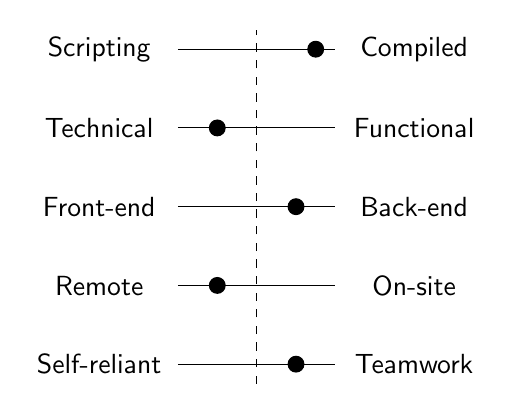
\begin{tikzpicture}
      \draw[dashed] (2, -0.25) -- (2, 4.25);
  
      \draw (1, 4) -- (3, 4);
      \filldraw (2.75, 4) circle (0.1);
      \node at (0, 4) {Scripting};
      \node at (4, 4) {Compiled};
  
      \draw (1, 3) -- (3, 3);
      \filldraw (1.5,3) circle (0.1);
      \node at (0,3) {Technical};
      \node at (4,3) {Functional};
  
      \draw (1, 2) -- (3, 2);
      \filldraw (2.5,2) circle (0.1);
      \node at (0,2) {Front-end};
      \node at (4,2) {Back-end};
  
      \draw (1, 1) -- (3, 1);
      \filldraw (1.5, 1) circle (0.1);
      \node at (0, 1) {Remote};
      \node at (4, 1) {On-site};
  
      \draw (1, 0) -- (3, 0);
      \filldraw (2.5,0) circle (0.1);
      \node at (0,0) {Self-reliant};
      \node at (4,0) {Teamwork};
    \end{tikzpicture}
  \end{figure}
  \vspace{0.75cm}

  % ------------------------------ Certifications ------------------------------ %
  \TitleTwo{\ColorHighlight}{\Large\faCertificate}{Certifications}
  \begin{ItemList}{\ColorHighlight}
    \item [\ding{226}] TOEIC:\@ 950 / 990
    \item [\ding{226}] Driver's license
    \item [\ding{226}] First aid in teams
  \end{ItemList}
  \vspace{0.5cm}

  % --------------------------------- Interests -------------------------------- %
  \TitleTwo{\ColorHighlight}{\Large\faHeart}{Interests}
  % \vspace{-\baselineskip}
  \begin{multicols}{2}
    \begin{ItemList}{\ColorHighlight}
      \item Martial arts
      \item Cycling
      \item Hiking
      \item Horse riding
    \end{ItemList}
  \end{multicols}
\end{SideBar}
\DefineProfile{\ColorOther}{\ColorTextSide}{img/profile_bw.jpg}
\begin{MainPart}
  \color{Black}
  \TitleOne{\ColorHighlight}{About me}{\faUser}
  \vspace{0.25cm}
  {
    \vspace{-\baselineskip}
    \begin{flushleft}
      Enthusiastic baby software engineer, I enjoy learning new things and tend to go `in depth' rather than `in breadth'. I began involving myself in conferences since 2022 and joined the Scala open-source community in 2023.

      Scala and functional programming are my current passions

      ArchLinux user, I enjoy using the command line (git included even though I sometimes need to hard-reset to clean up\dots)
    \end{flushleft}
  }
  
  % --------------------------------- Education -------------------------------- %
  \TitleOne{\ColorHighlight}{Education}{\faGraduationCap}
  \Experience%
  {\href{https://www.polytech.umontpellier.fr/images/ecole/Plaquettes/SPECIALITE_IG_2018_EN.pdf}{Engineering degree in Computer Science}}
  {\href{https://english.polytech.umontpellier.fr/}{Polytech Montpellier, France}}
  {2021 --- 2024}
  {
    Polytech Montpellier is a French engineering school at Montpellier, France.\\
    This degree is equivalent to a Master's degree
  }

  % -------------------------------- Main Skills ------------------------------- %
  \TitleOne{\ColorHighlight}{Main Skills}{\faStar}
  \vspace{0.3cm}

  \begin{minipage}{0.55\textwidth}
    \begin{description}
      \item[Paradigms] Functional, Object-oriented
      \item[Languages] Scala, Typescript, Java
      \item[Frameworks \& libraries] Nestjs, React
      \item[Databases] SQL (Postgres)
      \item[Tools \& Platforms] Git, GitHub, Docker
    \end{description}
  \end{minipage}
  \hfill
  \begin{minipage}{0.40\linewidth}
    \begin{tabular}{ccc}
      
\includegraphics[height=25pt]{img/scala-spiral.png} & 
\includegraphics[height=25pt]{img/typescript.png} & 
\includegraphics[height=25pt]{img/java.png}       \\
      
\includegraphics[height=25pt]{img/nestjs.png}       & 
\includegraphics[height=25pt]{img/react.png}      & 
\includegraphics[height=25pt]{img/postgresql.png} \\
      
\includegraphics[height=25pt]{img/git.png}          & 
\includegraphics[height=25pt]{img/github.png}     & 
\includegraphics[height=25pt]{img/docker.png}
    \end{tabular}
  \end{minipage}
  \vspace{0.3cm}

  % -------------------------------- Experiences ------------------------------- %
  \TitleOne{\ColorHighlight}{Experiences}{\faSuitcase}
  \Experience%
  {\href{https://github.com/scalacenter/scala-debug-adapter/pulls?q=is\%3Apr+author\%3Aiusildra+}{Software Engineer Intern (link)}}
  {Scala Center, EPFL}
  {Apr. 2023 --- Aug. 2023}
  {
    \textit{Scala, Git, JVM, Scala-Java Interoperability, Reflection}
    \begin{ItemList}{\ColorHighlight}
      \item[\ding{226}] Improved the Scala debugger in VS Code with a faster and more flexible evaluation mode
      \item[\ding{226}] Encountered problems similar to those of a compiler: type checking, types resolution, overloads resolution\dots
      \item[\ding{226}] I entend to keep upgrading it to make it more efficient, accepts more expressions, correct bugs\dots
    \end{ItemList}
  }
  \Experience%
  {Assistant Software Engineer}
  {Teads France}
  {Jun. 2022 --- Aug. 2022}
  {
    \textit{Scala, Cats-Effect, gRPC, MySQL, React (TS), Git, Cypress}

    \begin{ItemList}{\ColorHighlight}
      \item[\ding{226}] Full-stack development of the v2 of their demo application
      \item[\ding{226}] Handled each feature from the database to the UI (code, test, deploy)
    \end{ItemList}
  }
\end{MainPart}

\pagebreak

\leftframe%

% ---------------------------------------------------------------------------- %
%                                  Open source                                 %
% ---------------------------------------------------------------------------- %
\TitleOne{\ColorHighlight}{Open source}{\faCodeBranch}
\begin{multicols}{2}
  [\Experience{\href{https://github.com/scalacenter/scala-debug-adapter}{Scala Debuger Adapter}}{Scala Center \& personal time}{2023 --- .}{
      Implementation of the Scala debugger for VS Code \& follow up of my internship at the Scala Center.
    }]
  \Experience{\href{https://github.com/scala/scala}{Scala Collections}}{Personal time}{2023 --- .}{
    Joined the \texttt{scala-collections} team to review pull-requests on Scala's collections
  }

  \columnbreak{}

  \Experience{\href{https://github.com/lampepfl/dotty}{Scala 3 (Dotty)}}{Scala Center \& personal time}{2023 --- .}{
    Onboarded on the compiler with the \ul{\href{https://www.scala-lang.org/blog/2022/11/02/compiler-academy.html}{compiler academy}} to work on small issues.
  }

\end{multicols}



% ---------------------------------------------------------------------------- %
%                                 ASSOCIATIONS                                 %
% ---------------------------------------------------------------------------- %
\TitleOne{\ColorHighlight}{Associative}{\faIcon{share-alt}}

\begin{multicols}{2}
  [
    \Experience{Organizer}{Sunny Tech}{2022 --- .}{
      \begin{multicols}{2}
        \begin{ItemList}{\ColorHighlight}
          \item[\ding{72}] \ul{\href{https://sunny-tech.io}{https://sunny-tech.io}}
          \item[\ding{72}] Community Management (\ul{\href{https://www.linkedin.com/company/18442273}{LinkedIn}}, \ul{\href{https://twitter.com/SunnyTech_MTP}{Twitter}})
          \item[\ding{72}] Call For Papers reviewer (450 talks)
          \item[\ding{72}] 2023 --- 2024: Secretary
        \end{ItemList}
      \end{multicols}
    }
  ]
  \Experience{Organizer}{ScalaIO}{2023 --- .}{
    \begin{ItemList}{\ColorHighlight}
      \item[\ding{72}] \ul{\href{https://scala.io}{https://scala.io}}
      \item[\ding{72}] Call For Papers reviewer
    \end{ItemList}
    \null{}
  }
  \null{}
  \columnbreak{}
  \Experience{Volunteer}{Scala Days Madrid}{Sept. 2023}{
    \begin{ItemList}{\ColorHighlight}
      \item[\ding{72}] \ul{\href{https://scaladays.org/madrid-2023}{https://scaladays.org/madrid-2023}}
      \item[\ding{72}] Track hosting (speaker presentation, time + Q\&A management)
      \item[\ding{72}] Mentoring at \ul{\href{https://github.com/scalabridgelondon/scaladays-madrid-2023-scalabridge}{Scala Bridge}} (co-located event)
    \end{ItemList}
  }
  \null{}
\end{multicols}



% ---------------------------------------------------------------------------- %
%                                    OTHERS                                    %
% ---------------------------------------------------------------------------- %
\TitleOne{\ColorHighlight}{Others}{\faLaptopCode}
\begin{multicols}{2}
  \Experience{Website maintainer}{ScalaIO}{Dec. 2023 --- today}{
    \textit{Scala, Scala.js, Laminar, Sass, Github Actions, Clever Cloud}
    \vspace{0.25cm}
  
    Continued the work of the previous maintainer to rework the website with \ul{\href{https://www.scala-js.org}{Scala.js}} and \ul{\href{https://laminar.dev}{Laminar}} to build a reactive SPA (Single-Page Application) with Scala. Used \ul{\href{https://sass-lang.com}{Sass}} to style the website.
    \begin{ItemList}{\ColorHighlight}
      \item[\ding{226}] Github Actions
      \item[\ding{226}] Clever Cloud deployment
      \item[\ding{226}] Web apps performance metrics
    \end{ItemList}
  
    Github repo: \ul{\href{https://github.com/ScalaIO/scala.io}{https://github.com/ScalaIO/scala.io}}

    Website url: \ul{\href{https://scala.io}{https://scala.io}}
  }
  \vfill{}
  \null{}
  \columnbreak{}
  \Experience{Courses}{Polytech Montpellier}{Nov. 2023 --- .}{
    \textit{Functional Programming, Scala, Type Classes, Parsers}
    \vspace{0.25cm}
  
    Started with a 3h course about building parsers with functional programming (FP) to master students, based on the \ul{\href{https://www.creativescala.org/case-study-parser/index.html}{Parser combinators}} workshop from \ul{\href{https://github.com/noelwelsh}{Noel Welsh}}:
    \begin{ItemList}{\ColorHighlight}
      \item[\ding{226}] Reminders about Scala \& FP
      \item[\ding{226}] Design with Type Classes
      \item[\ding{226}] Frequent and small exercices
      \item[\ding{226}] \ul{\href{https://iusildra.github.io/reveal.js/presentations/functional-design-parser-combinators/index.html}{Slides available here}}
    \end{ItemList}
  
    \vspace{0.25cm}
    Starting from 2024 --- 2025, I'll give around a +9h course about functional programming in general, with Scala as base language, which will serve as a basis for another course given by someone else.
  }
  \vfill{}
  \null{}
\end{multicols}

\begin{tikzpicture}[remember picture,overlay]
  \node[anchor=south east,inner sep=7.5pt] at (current page.south east) {
\includegraphics[height=1.5cm]{img/archlinux.png}};
\end{tikzpicture}

\end{document}


